\section{Results}\label{sec:results}

% 이 절에서는 \ref{sec:methods}에서 소개한 모형들을 자료에 적용한 결과를 다룬다. 각 모형의 성능은 \citet{jeon2018additive}에서와 같이 다음과 같이 정의되는 10-fold average squared prediction error (ASPE) 값으로 비교하였다
% $$ ㅁㄹㄴㄹ $$
% . 

\begin{figure}
    \centering
    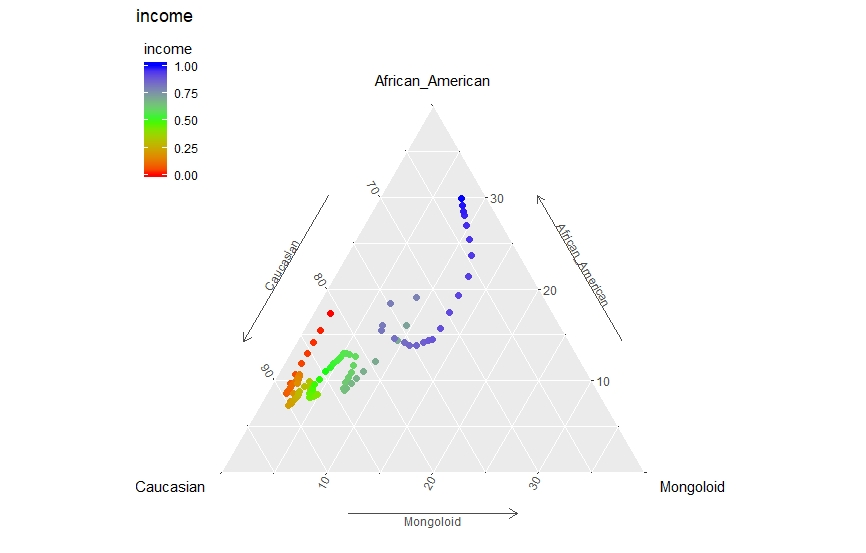
\includegraphics[width=0.7\textwidth]{figs/p_income.jpeg}
    \caption{TEST}\label{fig:test}
\end{figure}

Figure 1은 Jeon and Park(2018)에서 제시된 방법을 이용해서 적합한 성분비의 추정 값들이 각 요인들의 움직임에 따라 어떻게 움직이는지를 시각화한 것이다. 각각의 요인들의 영향력을 알아보기 위해서 우리는 성분비의 추정 값을 계산할 때 정해진 한 변수를 제외하고 다른 변수들은 모두 평균값으로 세팅하였고, 한 변수의 값을 움직임에 따라 어떻게 성분비의 추정 값이 분포되는 지를 분석해 보았다. 첫 번째 그림은 연령대가 변함에 따라서 인구 구성비 중에서 흑인과 백인의 비율이 두드러지게 변화한 다는 것을 알 수 있다. 연령대가 높아짐에 따라서 처음에는 백인의 비율이 감소하고 흑인의 비율은 증가하다가 일정 나이대를 지나면 다시 백인의 비율이 증가하고 흑인의 비율은 증가하는 경향을 보이고 있다. 여기서 동양인의 비율은 평균 연령대가 변화해도 크게 변동하지 않는 것이 흥미롭다. 두 번째 그림은 수입이 변화함에 따라서 인구 구성비가 어떻게 변화하는지를 보여주고 있다. 다른 4개의 요인에 비해서 많이 불규칙한 경향성을 보이고 있다. 다만 전반적으로 평균 수입이 늘어남에 따라서 동양인의 비율이 늘어나고 흑인의 비율은 줄어드는 경향을 보이고 있다. 또한, 일정 수준 이상부터는 수입이 늘어남에 따라 백인의 비율이 줄어드는 경향성을 보인다. 수입 최상위층 구간에서 흑인의 비율이 조금 늘어나고 동양인의 비율은 오히려 줄어드는 경향을 보이는 것은 흥미롭다. 세 번째 그림은 범죄율이 변함에 따라서 흑인과 백인의 비율이 두드러지게 변화하는 것을 알 수 있다. 양 극단을 제외하고는 범죄율이 높을수록 흑인의 비율이 늘어나고 백인의 비율은 줄어들지만, 극단에서는 이 관계가 역전이 되고 있다. 한편 동양인의 비율은 범죄율에 거의 영향이 없는 것으로 보인다. 네 번째 그림은 일정 온도 이하까지는 온도가 높아질수록 흑인의 비율은 늘어나고 백인의 비율은 줄어들다가 일정 온도 이상이 되면 흑인의 비율은 줄어들고 동양인의 비율은 두드러지게 늘어남을 알 수 있다. 이는 알래스카와 같은 척박한 곳에는 백인의 비율이 높지만 일정 온도 이상이 되면 온도가 오를 수록, 즉 살기에 더 쾌적할수록 동양인의 비율이 늘어나고 있음을 보여주고 있다. 다섯 번째 그림도 네 번째 그림과 비슷한 경향성을 보여준다. 즉 강수량이 낮은 구간에서는 백인의 비율이 높지만 일정 강수량 이상이 되는 지점부터는 강수량이 늘어날수록 동양인의 비율이 높아지고 있다.

% 실험과 관련된 코드는 github repository \url{https://github.com/kw-lee/ARHR_USA}에 제공되어 있다.

